\section{Linear complementary problem}
\subsection{Overview}
A linear complementary problem (LCP) is an optimization problem in which the goal is to solve a system of linear equations subject to a set of complementary conditions. More formally, given the matrix $\mathbf{A}\in\mathbb{R}^{d \times d}$ and the vector $\mathbf{b}\in\mathbb{R}^{d}$, find the vectors $\mathbf{v}\in\mathbb{R}^{d}$ and $\mathbf{w}\in\mathbb{R}^{d}$ such as
\begin{align*}
  \mathbf{A}\mathbf{v} - \mathbf{w} = \mathbf{b}
\end{align*}
subject to the complementary conditions 
\begin{align*}
  v_i &\ge 0 \qquad \text{for $i = 1,\dots,d$} \\
  w_i &\ge 0 \qquad \text{for $i = 1,\dots,d$} \\
  \mathbf{v}^{T}\mathbf{w} &= 0
\end{align*}
Note that the complementary conditions require that either $v_i=0$ or $w_i=0$. As you will see later, the pricing problem for American options can be reformulated as a linear complementary problem. Let us reconsider what the Black-Scholes model tells about American options. First, that the value $V(S,t)$ is bounded from below by the payoff function 
\begin{align*}
  V(S, t) - H(S, t) \ge 0 \qquad \text{for all $(S,t)$}
\end{align*}
Moreover, that the value function can be divided in two complementary regions: the exercise region \eqref{eq:blackscholes:preliminaries:exercise_region} where  
\begin{align}
  \label{eq:lcp:overview:value_in_continuation_region}
  &V(S, t) - H(S, t) > 0 \qquad \text{for $(S,t) \in \mathcal{C}$}
\end{align}
the continuation region \eqref{eq:blackscholes:preliminaries:continuation_region} where 
\begin{align}
  \label{eq:lcp:overview:value_in_exercise_region}
  &V(S, t) - H(S, t) = 0 \qquad \text{for $(S,t) \in \mathcal{S}$}
\end{align}
Finally, value function $V(S,t)$ is the solution to the Black-Scholes PDE  within the continuation region
\begin{align*}
    \frac{\partial{V}}{\partial{t}} + \mathcal{L}_{\text{BS}}(V) = 0 \qquad \text{for $(S,t) \in \mathcal{C}$}
\end{align*}
where $\mathcal{L}_{\text{BS}}(\cdot)$ is the linear parabolic operator \eqref{eq:blackscholes:preliminaries:linear_parabolic_operator} applied to the function $V(S,t)$. Now, let us consider what happens to the Black-Scholes PDE in the exercise region. From equation \eqref{eq:lcp:overview:value_in_exercise_region}, we know that $V(S,t)=H(S,t)$. Hence by plugin $H(S,t)$ into the Black-Scholes PDE, we obtain the Black-Scholes PDE inequality in the exercise region
\begin{align}
    \label{eq:lcp:overview:blackscholes_in_exercise_region}
    \frac{\partial{V}}{\partial{t}} + \mathcal{L}_{\text{BS}} \le 0 \qquad \text{for $(S,t) \in \mathcal{S}$}
\end{align}
By grouping \eqref{eq:lcp:overview:value_in_continuation_region}, \eqref{eq:lcp:overview:value_in_exercise_region}, \eqref{eq:lcp:overview:blackscholes_in_exercise_region}, we form the system of variational inequalities
\begin{align}
  \begin{cases}
    \big[\frac{\partial V}{\partial \tau} - \mathcal{L}_{\text{BS}}(V)\big] \cdot [V(S,T-\tau) - H(S,T-\tau)] = 0 & \text{for all $(S,t)$} \\
    V(S, T-\tau) - H(S, T-\tau) \ge 0 & \text{for all $(S, t) \ $}\\
    \frac{\partial V}{\partial \tau} - \mathcal{L}_{\text{BS}}(V) \ge 0 &  \text{for all $(S, t)$}\\
    V(S, T) = H(S, T) \\  
  \end{cases}
  \label{eq:lcp:overview:variational_inequalities}
\end{align}
The benefit of the variational inequalities is that there is no explicit dependence on the optimal exercise price defined in \eqref{eq:blackscholes:preliminaries:optimal_exercise_boundary}. Also, note that we rewrote the Black-Scholes PDE forward in time by introducing the transformation $\tau = T - t$ deliberately so that the variational inequalities' formulation looks similar in structure to LCP problem. But before elaborating more about the relationship between the variational inequalities and LCP problems, we introduce the transformations
\begin{align}
\label{eq:lcp:overview:heat_diffusion_domain_transformation}
S = Ke^x, \quad t = T - \dfrac{2\tau}{\sigma^2},\quad h(x,\tau) := e^{(\alpha x + \beta \tau)}\dfrac{H(S,t)}{K}, \quad v(x, \tau) := V(S, t) =: Ke^{-(\alpha x + \beta \tau)}y(x, \tau)
\end{align}
where
\begin{align}
  \label{eq:lcp:overview:heat_diffusion_domain_transformation_2}
  q &:= \dfrac{2r}{\sigma^2}, \quad q_{\delta} := \dfrac{2(r-\delta)}{\sigma^2}, \quad \alpha := \dfrac{1}{2}(q_{\delta} - 1) \quad \beta := \dfrac{1}{4}(q_{\delta} - 1)^2 + q 
\end{align}
so that the Black-Scholes PDE \eqref{eq:chapter2:european_option_pde_with_dividens} transforms to the heat diffusion equation
\begin{align}
  \label{eq:lcp:overview:heat_diffusion_equation_PDE}
  \dfrac{\partial{y}}{\partial{\tau}} - \dfrac{\partial^2{y}}{\partial{x^2}} = 0
\end{align}
where $y\in C^{2,1}(\mathcal{F})$ for
\begin{align}
  \label{eq:lcp:overview:heat_diffusion_equation_solution_region}
  \mathcal{F}: \mathbb{R} \times [0, \sigma^2T/2]
\end{align}
Although we might solve \eqref{eq:lcp:overview:variational_inequalities} without transforming the problem, Dewynne et al. \cite{dewynne_howison_rupf_wilmott_1993} and Seydel \cite{seydel_2009} suggest that transformation to the heat diffusion equation \eqref{eq:lcp:overview:heat_diffusion_equation_PDE} introduces desirable numerical properties when applying finite difference schemes. By applying transformation \eqref{eq:lcp:overview:heat_diffusion_domain_transformation}, the system \eqref{eq:lcp:overview:variational_inequalities} becomes
\begin{align}
  \begin{cases}
    \bigg[\dfrac{\partial{y}}{\partial{\tau}} - \dfrac{\partial^2{y}}{\partial{x^2}}\bigg] \cdot [y(x, \tau) - h(x, \tau)] = 0 & \text{for all $(x,\tau)$} \\
    y(x, \tau) - h(x, \tau) \ge 0 & \text{for all $(x, \tau)$}\\
    \dfrac{\partial{y}}{\partial{\tau}} - \dfrac{\partial^2{y}}{\partial{x^2}} \ge 0 &  \text{for all $(x, \tau)$}\\
    y(x, 0) = h(x, 0) \\  
  \end{cases}
  \label{eq:lcp:overview:variational_inequalities_heat_equation}
\end{align}
Now that we have expressed the system of variational inequalities using the heat discussion equation, we proceed to apply the finite difference scheme framework presented in section \ref{sec:finitedifferencesschemes}. Specifically, we want to approximate $y(x, \tau)$ at each of the nodes within the grid 
\begin{align}
  \mathcal{G} := \{(x_i, \tau_n): (i, n) \in \{0, \dots, M+1\} \times \{0, \dots, N+1\}\}
\end{align}
where 
\begin{align}
  \label{eq:lcp:overview:grid_2}
  x_i &:= x_{\text{min}} + i\Delta{x} &  \qquad \text{for $i = 0,\dots, M+1$} \\
  \tau_n &:= t_{\text{min}} + i{\Delta{\tau}} & \qquad \text{for $i = 0,\dots, N+1$} \\
  \Delta{x} &:= \dfrac{x_{\text{max}} - x_{\text{min}}}{M+1} \\ 
  \Delta{t} &:= \dfrac{t_{\text{max}} - t_{\text{min}}}{N+1}
\end{align}
where $x_{\text{min}}$ is set sufficiently small value, $x_{\text{max}}$ to a sufficiently large value, $\tau_{\text{min}}$ to 0 and $\tau_{\text{max}}$ to $\dfrac{\sigma^2}{2}T$. Recall that we presented explicit and implicit schemes for approximating the PDE \eqref{eq:blackscholes:frontfixingmethod:nielsen:american_options_pde} in section \ref{sec:finitedifferencesschemes}. Analogously, we present explicit and implicit schemes for the heat diffusion equation
\begin{align}
  \label{eq:lcp:overview:explicit_scheme}
  \dfrac{y^{n+1}_{i} - y^{n}_{i}}{\Delta \tau} =& \dfrac{y^{n}_{i-1} - 2y^{n}_{i} + y^{n}_{i+1}}{(\Delta x)^2}\\
  \label{eq:lcp:overview:implicit_scheme}
  \dfrac{y^{n+1}_{i} - y^{n}_{i}}{\Delta \tau} =& \dfrac{y^{n+1}_{i-1} - 2y^{n+1}_{i} + y^{n+1}_{i+1}}{(\Delta x)^2}
\end{align}
for $i=1,\dots,M$ and $n=0\dots,N$. Note that contrary to \eqref{eq:blackscholes:frontfixingmethod:nielsen:american_options_pde}, the heat equation is written forward in time. Therefore, the explicit scheme correspond to equation \eqref{eq:lcp:overview:explicit_scheme}, and the implicit scheme to equation \eqref{eq:lcp:overview:implicit_scheme}. In addition, we introduce the Crank-Nicholson scheme\cite{epperson_2013}\cite{seydel_2009} for equation \eqref{eq:lcp:overview:heat_diffusion_equation_PDE} as 
\begin{equation}
  \label{eq:lcp:overview:crank_nicholson}
  \dfrac{y^{n+1}_{i} - y^{n}_{i}}{\Delta \tau} = \dfrac{1}{2}\bigg(\dfrac{y^{n}_{i-1} - 2y^{n}_{i} + y^{n}_{i+1}}{(\Delta x)^2} + \dfrac{y^{n+1}_{i-1} - 2y^{n+1}_{i} + y^{n+1}_{i+1}}{(\Delta x)^2}\bigg)
\end{equation}
for $i=1,\dots,M$ and $n=0\dots,N$. Epperson \cite{epperson_2013} and Seydel \cite{seydel_2009} showed that the Crank-Nicholson scheme is $O(\Delta{x}^2 + \Delta{t}^2)$.
\begin{figure}[H]
  \label{fig:lcp:thetamethod:stencil}
  \centering
  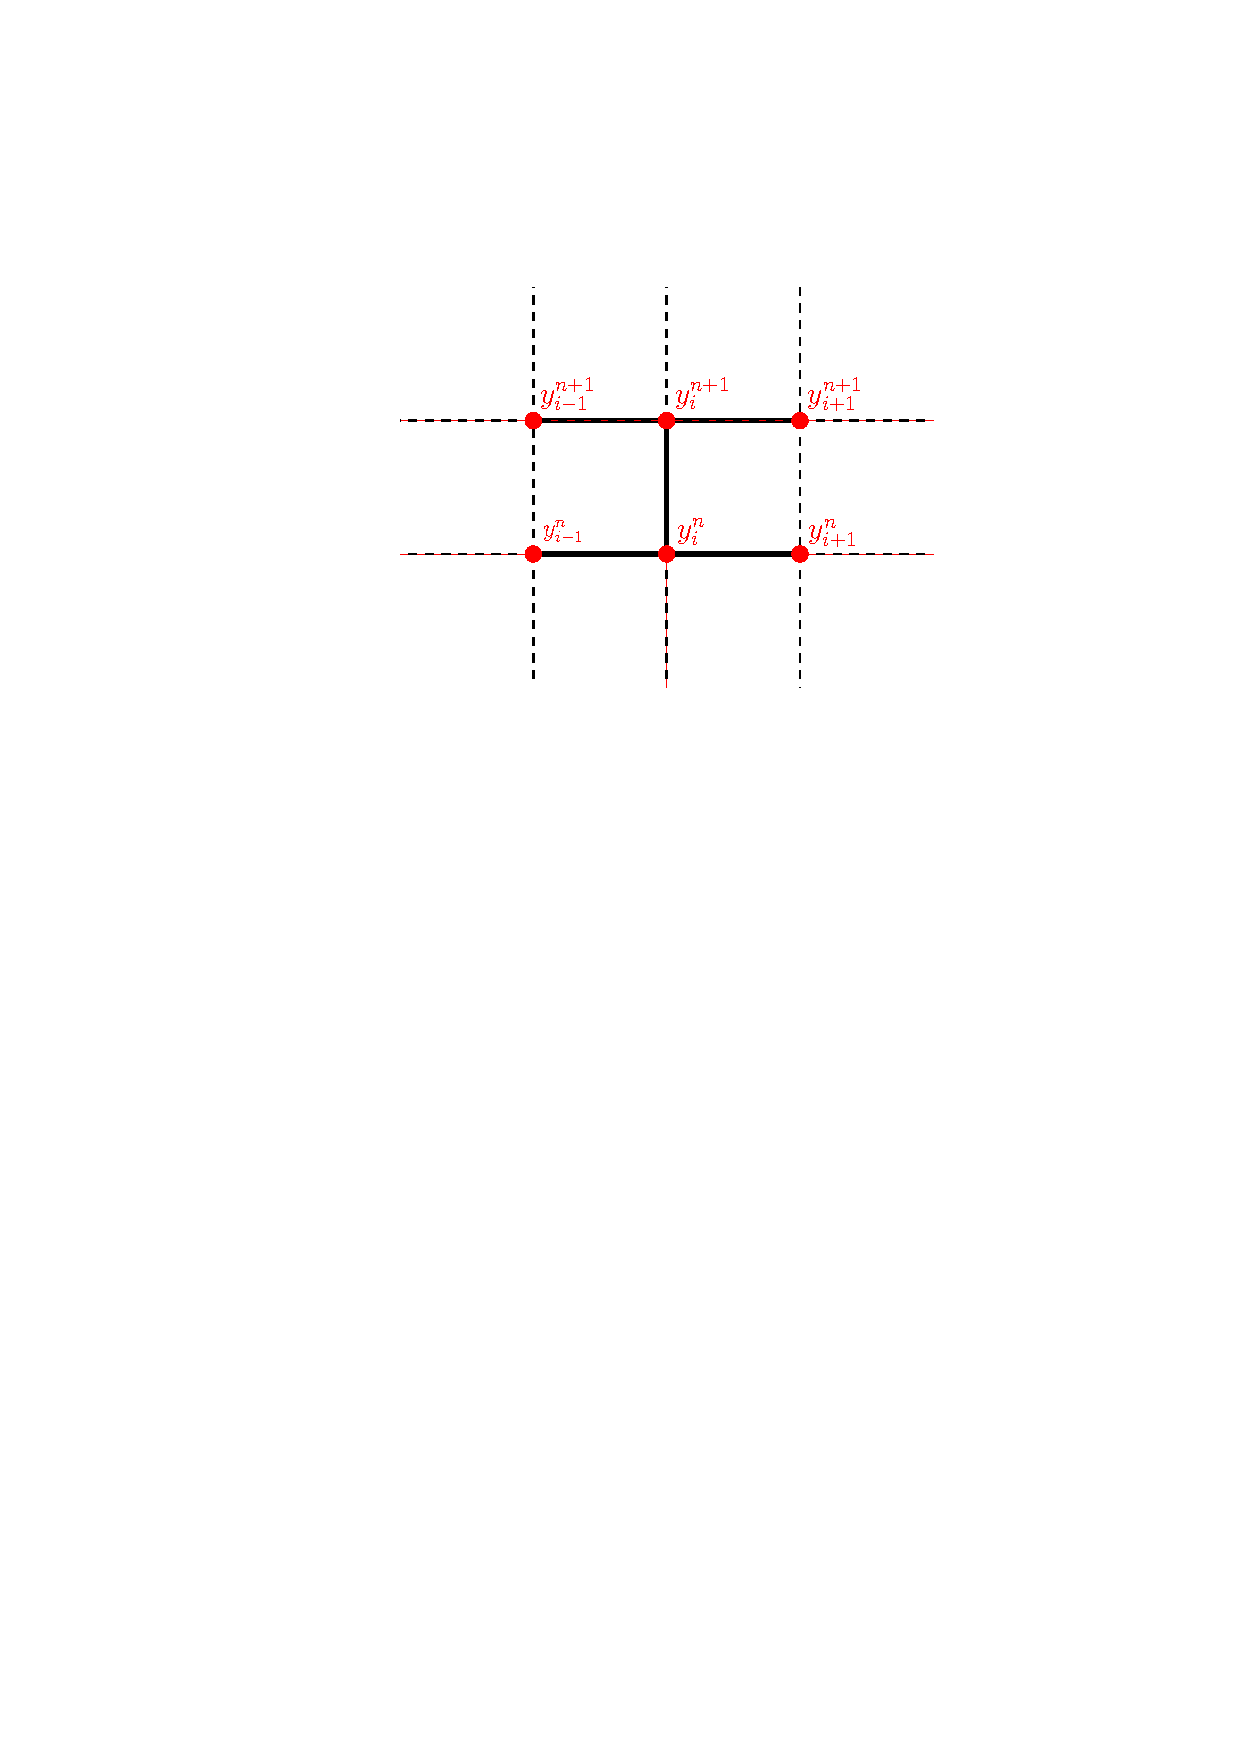
\includegraphics[scale=0.75]{chapters/chapter5/CrankNicholsonStencil.pdf}
  \caption{Stencil diagram for the Crank-Nicholson scheme.}
\end{figure} 
We can generalize \eqref{eq:lcp:overview:explicit_scheme}, \eqref{eq:lcp:overview:implicit_scheme}, and \eqref{eq:lcp:overview:crank_nicholson} using a parametrized scheme called the theta method 
\begin{equation}
  \label{eq:lcp:overview:theta_method}
  \dfrac{y^{n+1}_{i} - y^{n}_{i}}{\Delta \tau} = (1-\theta)\dfrac{y^{n}_{i-1} - 2y^{n}_{i} + y^{n}_{i+1}}{(\Delta x)^2} + \theta\dfrac{y^{n+1}_{i-1} - 2y^{n+1}_{i} + y^{n+1}_{i+1}}{(\Delta x)^2}
\end{equation}
for $i = 1,\dots,M$, and $n = 0,\dots,N$. The parameter $\theta\in[0,1]$ controls what scheme to use. The scheme defaults to the explicit method when $\theta=0$, to the implicit method when $\theta=1$, to the Crank-Nicholson when $\theta=1/2$. Next, we rearrange equation \eqref{eq:lcp:overview:theta_method} as
\begin{equation}
  \label{eq:lcp:thetamethod:finitedifference_approximation_2}
  y^{n+1}_{i} - \lambda\theta(y^{n+1}_{i-1} - 2y^{n+1}_{i} + y^{n+1}_{i+1}) =  y^{n}_{i} + (1-\theta)\lambda(y^{n}_{i-1} - 2y^{n}_{i} + y^{n}_{i+1})
\end{equation}
for $i = 1,\dots,M$, $n = 0,\dots,N$, and $\lambda=\Delta{t}/\Delta{x}^2$. Moreover, let us define vectors $\hat{\mathbf{b}}^n\in\mathbb{R}^{M}$, $\mathbf{y}^{n+1}\in\mathbb{R}^{M}$ and $\mathbf{h}^n\in\mathbb{R}^{M}$ as
\begin{align}
  \label{eq:lcp:thetamethod:b_hat}
  \hat{\mathbf{b}}^{n} :=& \begin{bmatrix}
    \hat{b}^{n}_1, \dots, \hat{b}^{n}_{M}
  \end{bmatrix}^{\textbf{T}}\\
  \mathbf{y}^{n+1} :=& \begin{bmatrix}
    y^{n+1}_1, \dots, y^{n+1}_{M}
  \end{bmatrix}^{\textbf{T}}\\
  \label{eq:lcp:thetamethod:h_vector}
  \mathbf{h}^{n+1} :=& \begin{bmatrix}
    h(x_1, \tau_{n+1}), \dots, h(x_M, \tau_{n+1})
  \end{bmatrix}^{\textbf{T}}
\end{align}
where 
\begin{equation}
  \hat{b}^{n}_i := y^{n}_{i} + (1-\theta)\lambda(y^{n}_{i-1} - 2y^{n}_{i} + y^{n}_{i+1})
\end{equation}
for $i = 1,\dots,M$, and $n = 0,\dots,N$. Finally, we define the matrix $\mathbf{A}\in\mathbb{R}^{M \times M}$ as
\begin{align}
  \label{eq:lcp:overview:theta_matrix}
  A :=& \begin{bmatrix}
    1+2\lambda\theta & -\lambda\theta & & 0 \\ 
   -\lambda\theta & \ddots & \ddots \\
      & \ddots & \ddots & \ddots \\
    0 & & \ddots & \ddots & \\
  \end{bmatrix} 
\end{align}
Hence, using vectors $\hat{\mathbf{b}}^n\in\mathbb{R}^{M}$, $\mathbf{y}^{n+1}\in\mathbb{R}^{M}$ and $\mathbf{h}^n\in\mathbb{R}^{M}$, and the matrix $\mathbf{A}\in\mathbb{R}^{M \times M}$, we could rewrite the system of variational inequalities \eqref{eq:lcp:overview:variational_inequalities_heat_equation}using the finite difference scheme proposed as
\begin{align}
  \label{eq:lcp:overview:variational_inequalities_fd}
  \begin{cases}
    (\mathbf{A}\mathbf{y}^{n+1} - \hat{\mathbf{b}}^{n})^{\text{T}}(\mathbf{y}^{n+1}- \mathbf{h}^{n+1}) = 0\\
    \mathbf{A}\mathbf{y}^{n+1} - \hat{\mathbf{b}}^{n} \ge 0\\
    \mathbf{y}^{n+1}- \mathbf{h}^{n+1} \ge 0\\
    \mathbf{y}^{0} = \mathbf{h}^{0}
  \end{cases}
\end{align}
for $n=0,\dots,N$. Moreover, \eqref{eq:lcp:overview:variational_inequalities_fd} can be formulated as the iterative method
\begin{algorithm}[H]
  \caption{Iterative method for variational inequalities.}\label{alg:lcp:overview:variational_inequalities_iterative_method}
  \begin{algorithmic}
  \State $\mathbf{y}^{0} = \mathbf{h}^{0}$
  \For{$n = 0,\dots,N$} 
  \State Find $\mathbf{y}^{n+1}$ such as 
  \State $\qquad (\mathbf{A}\mathbf{y}^{n+1} - \hat{\mathbf{b}}^{n})^{\text{T}}(\mathbf{y}^{n+1}- \mathbf{h}^{n+1}) = 0$
  \State $\qquad \mathbf{A}\mathbf{y}^{n+1} - \hat{\mathbf{b}}^{n} \ge 0$
  \State $\qquad \mathbf{y}^{n+1}- \mathbf{h}^{n+1} \ge 0$
  \EndFor
\end{algorithmic}
\end{algorithm}
\newpage
Finally, by defining $\mathbf{v} := \mathbf{y}^{n+1} - \mathbf{h}^{n+1}$,  $\mathbf{w} := \mathbf{A}\mathbf{y}^{n+1} - \hat{\mathbf{b}}^{n}$, $\mathbf{b} := \hat{\mathbf{b}}^n - \mathbf{A}\mathbf{h}^{n+1}$. The iterative \ method becomes
\begin{algorithm}[H]
  \caption{Iterative method for LCP.}\label{alg:lcp:overview:lcp_iterative_method}
  \begin{algorithmic}
  \For{$n = 0,\dots,N$} 
  \State Given $\mathbf{A}\mathbf{v} - \mathbf{w} = \mathbf{b}$, find $\mathbf{v}$ and $\mathbf{w}$ such as 
  \State $\qquad \mathbf{v} \ge 0$
  \State $\qquad \mathbf{w} \ge 0$
  \State $\qquad \mathbf{v}^{\text{T}}\mathbf{w} \ge 0$
  \EndFor
\end{algorithmic}
\end{algorithm}
Note, that solving the variational inequalities is equivalent to solve an LCP problem for $n=0,\dots,N$.
\subsection{PSOR method}
The LCP reformulation for the pricing problem requires to solve a system of linear equations subject to complementary conditions. Therefore, we consider the problem of solving the linear equation $\mathbf{A}\mathbf{x}=\mathbf{b}$ for $\mathbf{A}\in\mathbb{R}^n$, and $\mathbf{b}\in\mathbb{R}^n$. Suppose that $\mathbf{M} = \mathbf{A} + \mathbf{N}$ is a non-singular matrix. Then, the linear equation can be rewritten as
\begin{align}
  \mathbf{M}\mathbf{x}=\mathbf{N}\mathbf{x} + \mathbf{b}
\end{align}
or as 
\begin{align}
  \label{eq:lcp:psor:fix_point_equation}
  \mathbf{x} = \mathbf{B}\mathbf{x} + \mathbf{M}^{-1}\mathbf{b}
\end{align}
where $\mathbf{B} := \mathbf{M}^{-1}\mathbf{N} = \mathbf{I}-\mathbf{M}^{-1}\mathbf{A}$. Clearly, equation \eqref{eq:lcp:psor:fix_point_equation} constitute fixed-point problem\cite{epperson_2013} which leads to the iterative method
\begin{align}
  \label{eq:lcp:psor:fix_point_iterative}
  \mathbf{x}^{k} = \mathbf{B}\mathbf{x}^{k-1} + \mathbf{M}^{-1}\mathbf{b}
\end{align}
Epperson\cite{epperson_2013} showed that iterative method \eqref{eq:lcp:psor:fix_point_iterative} converges given an initial guess $\mathbf{x}^{0}$ when
\begin{align*}
  \rho(\mathbf{B}) < 1
\end{align*}
where $\rho(\mathbf{B})$ is the spectral radius of matrix $\mathbf{B}$. Different choices of matrix $\mathbf{M}$ will yield to different methods with different convergence rate. The Jacobi method defines $\mathbf{M}$ and $\mathbf{N}$ such as $\mathbf{A}=\mathbf{M}-\mathbf{N}=\mathbf{D} - (\mathbf{L} + \mathbf{U})$, yielding the iterative method
\begin{align}
  \mathbf{D}\mathbf{x}^{k} = (\mathbf{L} + \mathbf{U})\mathbf{x}^{k-1} + \mathbf{M}^{-1}\mathbf{b}
\end{align}
According to Epperson\cite{epperson_2013}, the Jacaobi method has the slowest convergence of all the other iterative methods that we could come with. Similarly, the Gauss-Seidel method is given by defining $\mathbf{M} := \mathbf{D} - \mathbf{L}$ and $\mathbf{N}:=\mathbf{U}$.
\begin{align}
  \label{eq:lcp:psor:gauss_seydel}
  (\mathbf{D} - \mathbf{L})\mathbf{x}^{k} = \mathbf{U}\mathbf{x}^{k-1} + \mathbf{M}^{-1}\mathbf{b}
\end{align}
A generalization of the Gauss-Seidel \eqref{eq:lcp:psor:gauss_seydel} method is given by is the successive over-relaxation (SOR) method. The SOR method defines $M$ and $N$ as 
\begin{align*}
  \mathbf{M} := \frac{1}{\omega}\mathbf{D} - \mathbf{L}, \qquad \mathbf{N}=\bigg(\frac{1}{\omega} -1\bigg)\mathbf{D} + \mathbf{U}
\end{align*}
where $\omega$ is the relaxation parameter. Thus, resulting in the iterative method
\begin{align}
  \label{eq:lcp:psor:sor_method}
  \bigg(\frac{1}{\omega}\mathbf{D} - \mathbf{L}\bigg)\mathbf{x}^{k} = \bigg(\bigg(\frac{1}{\omega}-1\bigg)\mathbf{D} + \mathbf{U}\bigg)\mathbf{x}^{k-1} + \mathbf{b}
\end{align}
Note that for $\omega=1$, the Gauss-Seidel \eqref{eq:lcp:psor:sor_method} method is obtained. Suppose, we want to solve $\mathbf{A}\mathbf{v}=\mathbf{b}$ for $\mathbf{A}$ given as in \eqref{eq:lcp:overview:theta_matrix}, $\mathbf{v}\in\mathbb{R}^{M}$, and $\mathbf{b}\in\mathbb{R}^{M}$. Then, a componentwise version of the \eqref{eq:lcp:psor:sor_method} is given by 
\begin{align}
  \label{eq:lcp:psor:sor_method_cwise}
  \frac{1}{\omega}(1+2\alpha)v^{k}_i = \bigg(\frac{1}{\omega}-1\bigg)(1+2\alpha)v^{k-1}_{i} + \alpha (v^{k}_{i-1} + v^{k-1}_{i+1}) + b_i
\end{align}
for $\alpha=\lambda\theta$ and $i=1,\dots,M$. Moreover, an iterative algorithm will be given as
\begin{algorithm}[H]
  \caption{SOR for the theta method.}\label{alg:lcp:overview:sor_method_theta}
  \begin{algorithmic}[1]
  \For{$k = 1,\dots$} 
  \For{$i = 1,\dots, M$}
  \State $r^{k}_{i} = (\alpha(v^{k}_{i-1} + v^{k-1}_{i+1}) + b_i)/(1+2\alpha)$ 
  \State $v^{k}_{i} = v^{k-1}_i + \omega(r^{k}_{i} - v^{k-1}_i)$
  \EndFor
  \EndFor
\end{algorithmic}
\end{algorithm}
The project SOR (PSOR) method is a slight modification of SOR method in which the positivity of $v^{k}_i$ is enforced at line number 5 of \eqref{alg:lcp:overview:sor_method_theta}.
\begin{algorithm}[H]
  \caption{PSOR for the theta method.}\label{alg:lcp:overview:psor_method_theta}
  \begin{algorithmic}[1]
  \For{$k = 1,\dots$} 
  \For{$i = 1,\dots, M$}
  \State $r^{k}_{i} = (\alpha(v^{k}_{i-1} + v^{k-1}_{i+1}) + b_i)/(1+2\alpha)$ 
  \State $v^{k}_{i} = \max\big\{0, v^{k-1}_i + \omega(r^{k}_{i} - v^{k-1}_i)\big\}$
  \EndFor
  \EndFor
\end{algorithmic}
\end{algorithm}
Moreover, Seydel et al. \cite{seydel_2009} and Dewynne et al. \cite{wilmott_howison_dewynne_1995} showed that the PSOR method is equivalent to LCP algorithm \eqref{alg:lcp:overview:lcp_iterative_method}. Moreover, they also showed that the fasted convergence is given by having $\omega=1$. Putting algorithm \eqref{alg:lcp:overview:variational_inequalities_iterative_method}, \eqref{alg:lcp:overview:lcp_iterative_method} and \eqref{alg:lcp:overview:psor_method_theta} together, we have
\begin{algorithm}[H]
  \caption{Iterative method for solving heat diffusion variational inequalities.}\label{alg:lcp:psor:amer_option_solution}
  \begin{algorithmic}[1]
  \State Define $h(x,\tau)$ as in \eqref{eq:lcp:overview:heat_diffusion_domain_transformation}.
  \State Define grid as in \eqref{eq:lcp:overview:grid_2}.
  \State Set $\omega$ to 1.
  \State Set $\epsilon$ to some value closes to zero.
  \State $\mathbf{y}^{n}=h(x_i, 0)$ for $i=1,\dots,M$
  \For{$n = 0,\dots,N$} \Comment{Beginning of LCP problem}
    \State Define $\mathbf{h}^{n+1}$ as in \eqref{eq:lcp:thetamethod:b_hat}.
    \State Define $\hat{\mathbf{b}}^n$ as in \eqref{eq:lcp:thetamethod:h_vector}.
    \State $v^{0}_{i} := \max(y^{n}_i, h^{n+1}_i) \quad \text{for $i=1,\dots,M$}$\Comment{Beginning of PSOR method}
    \For{$k = 1,\dots$} 
    \For{$i = 1,\dots, M$}
    \State $r^{k}_{i} := (\alpha(v^{k}_{i-1} + v^{k-1}_{i+1}) + b_i)/(1+2\alpha)$ 
    \State $v^{k}_{i} := \max\big\{0, v^{k-1}_i + \omega(r^{k}_{i} - v^{k-1}_i)\big\}$
    \EndFor
    \If {$||\mathbf{v}^{k}-\mathbf{v}^{k-1}||_{2} \le \epsilon$}
      \State $\mathbf{v}^{\text{new}} := \mathbf{v}^{k}$
      \State Break out of the loop
    \EndIf
    \EndFor
    \State $\mathbf{y}^{n+1} :=\mathbf{v}^{k}$
  \EndFor
\end{algorithmic}
\end{algorithm}

\section{Numerical results}